

%-------------------------------------------------------------------------------
% Dokumenten Klasse
\documentclass[
	final,
	a4paper,
	oneside,
	parskip=full,
	headings=standardclasses,
	headings=big,
	pointednumbers
]{scrartcl}

%-------------------------------------------------------------------------------
% Packete nutzen
\usepackage[T1]{fontenc}
\usepackage[utf8]{inputenc}
\usepackage[left=15mm,right=20mm,top=15mm,bottom=15mm]{geometry}
\usepackage{amsmath}
\usepackage{amssymb}
\usepackage{mathtools}
\usepackage{mathtools}

%-------------------------------------------------------------------------------
% xcolor
\usepackage[svgnames]{xcolor}

%-------------------------------------------------------------------------------
% tabularx
\usepackage{tabularx}
\usepackage{ltablex}
\usepackage{makecell}

%-------------------------------------------------------------------------------
% TikZ
\usepackage{tikz}
\usetikzlibrary{positioning, arrows, decorations, calc, fit, intersections}

%-------------------------------------------------------------------------------
% Listings
\usepackage{listings}
\newcommand{\listingMatlab}[2][]{
	\lstset{
		language=Matlab,
		breaklines=true,
		numbers=left,
		numberstyle=\tiny,
		numbersep=5pt,
		captionpos=b,
		basicstyle=\footnotesize\ttfamily,
		stringstyle=\color{magenta},
		identifierstyle=\color{black},
		keywordstyle=\color{blue}, 
		commentstyle=\color{DarkGreen}
	}
	\lstinputlisting[caption={\texttt{\detokenize{#2}}},#1]{#2}
}
\lstnewenvironment{algorithm}[1][] %defines the algorithm listing environment
{
    \lstset{ %this is the stype
        mathescape=true,
        frame=tB,
        numbers=left, 
        numberstyle=\tiny,
        basicstyle=\scriptsize, 
        keywordstyle=\color{black}\bfseries,
        keywords={,input, output, return, datatype, function, in, if, else, foreach, while, begin, end, } 
        numbers=left,
        xleftmargin=.04\textwidth
    }
}
{}

%-------------------------------------------------------------------------------
% 
\newcommand{\f}[2]{\frac{#1}{#2}}
\newcommand{\fs}[2]{{\tfrac{#1}{#2}}}

% kl = ()
\newcommand{\kl}[1]{{\left( #1 \right)}}

% kq = {}
\newcommand{\kq}[1]{{\left\{ #1 \right\}}}

% ks = []
\newcommand{\ks}[1]{{\left[ #1 \right]}}

% 
\newcommand{\abs}[1]{{\vert #1 \vert}}

\newcommand\addvmargin[1]{
  \node[fit=(current bounding box),inner ysep=#1,inner xsep=0]{};
}

\def\tiktop{%
    \def\xlines{25}
    \def\ylines{15}
    \def\raster{3.5mm}

    \coordinate (P1S) at (0*\raster,14*\raster);
    \coordinate (P1E) at (24*\raster,6*\raster);

    \coordinate (P2S) at (1*\raster,6*\raster);
    \coordinate (P2E) at (11*\raster,4*\raster);

    \coordinate (P3S) at (3*\raster,7*\raster);
    \coordinate (P3E) at (15*\raster,15*\raster);

    \coordinate (P4S) at (5*\raster,9*\raster);
    \coordinate (P4E) at (14*\raster,10*\raster);

    \coordinate (P5S) at (8*\raster,1*\raster);
    \coordinate (P5E) at (23*\raster,8*\raster);

    \coordinate (P6S) at (16*\raster,6*\raster);
    \coordinate (P6E) at (20*\raster,5*\raster);

    % draw vertical lines
    \foreach \x in {0,...,\xlines}
    {
        \draw[lightgray] (\x * \raster, 0mm) -- (\x * \raster, \ylines * \raster);
    }

    % draw horizontal lines
    \foreach \y in {0,...,\ylines}
    {
        \draw[lightgray] (0mm, \y * \raster) -- (\xlines * \raster, \y * \raster);
    }

    % border
    \draw[black] (0mm, 0mm) -- (\xlines * \raster, 0mm);
    \draw[black] (0mm, 0mm) -- (0mm, \ylines * \raster);
    \draw[black] (\xlines * \raster, 0mm) -- (\xlines * \raster, \ylines * \raster);
    \draw[black] (0mm, \ylines * \raster) -- (\xlines * \raster, \ylines * \raster);

    % status
    \draw[black] (-1.5*\raster, 0mm) rectangle (-0.25*\raster, \ylines * \raster);

    % event queue
    \draw[black] (-1.5*\raster, -1.5*\raster) rectangle (\xlines * \raster, -0.25*\raster);
}

\def\Lupper{\mathcal{L}_{\mathrm{upper}}}
\def\Llower{\mathcal{L}_{\mathrm{lower}}}

\def\pich{6.5cm}
\def\picb{9cm}

\begin{document}

    \begin{tabularx}{\textwidth}{ll}
        % --- LINE 1 --------------------------------------------------------
        \noindent\parbox[c][\pich]{\picb}{
        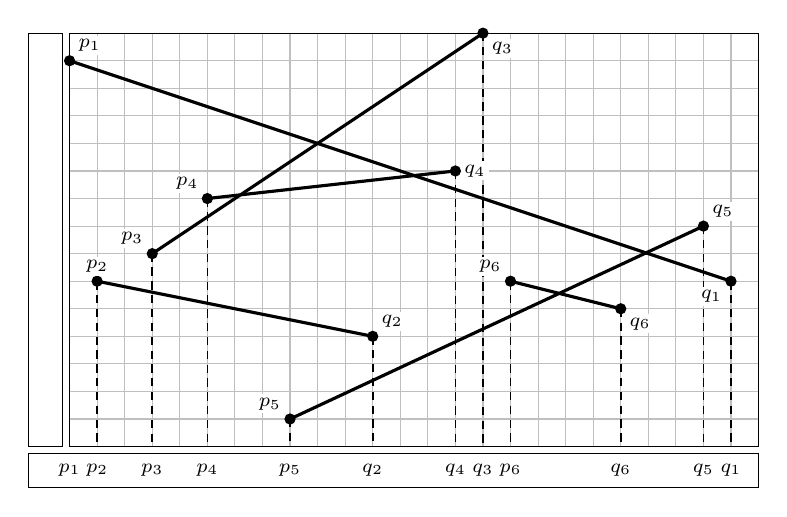
\begin{tikzpicture}[baseline=0]
            \tiktop
            
            -- line segments
            \foreach \start/\end in {
                P1S/P1E,
                P2S/P2E,
                P3S/P3E,
                P4S/P4E,
                P5S/P5E,
                P6S/P6E}
            {
                \draw[black,fill=black,line width=0.4mm]
                    (\start) -- (\end);
            }

            -- dashed lines
            \foreach \point in {
                P1S,P1E,
                P2S,P2E,
                P3S,P3E,
                P4S,P4E,
                P5S,P5E,
                P6S,P6E}
            {
                \draw[black,line width=0.2mm, densely dashed]
                    let
                        \p1 = (\point)
                    in
                        (\x1, \y1) -- (\x1, 0);
            }

            -- start- / end-point
            \foreach \point/\co in {
                P1S/black,P1E/black,
                P2S/black,P2E/black,
                P3S/black,P3E/black,
                P4S/black,P4E/black,
                P5S/black,P5E/black,
                P6S/black,P6E/black}
            {
                \draw[\co,fill=\co,line width=0.4mm]
                    (\point) circle (0.5mm);
            }

            -- events
            \foreach \event/\name/\i in {
                P1S/p/1,P1E/q/1,
                P2S/p/2,P2E/q/2,
                P3S/p/3,P3E/q/3,
                P4S/p/4,P4E/q/4,
                P5S/p/5,P5E/q/5,
                P6S/p/6,P6E/q/6}
            {
                \path
                    let
                        \p1 = (\event)
                    in 
                        node at (\x1,0) [below, fill=white, inner sep=1.25, outer sep=5] {$\scriptstyle \name_{\i} $};
            }

            -- start- / end-point text
            \foreach \point/\name/\i/\align/\co in {
                P1S/p/1/above right/black, P1E/q/1/below left/black,
                P2S/p/2/above/black,       P2E/q/2/above right/black,
                P3S/p/3/above left/black,  P3E/q/3/below right/black,
                P4S/p/4/above left/black,  P4E/q/4/right/black,
                P5S/p/5/above left/black,  P5E/q/5/above right/black,
                P6S/p/6/above left/black,  P6E/q/6/below right/black}
            {
                \node[\align, \co, fill=white, inner sep=1.25, outer sep=2] at (\point) {$\scriptstyle \name_{\i} $};
            }
        \end{tikzpicture}} &
        \makecell[l]{$\!\begin{aligned}[t]
            s_i     &= \text{Line segment} \\
            p_i     &= \text{Upper endpoint} \\
            q_i     &= \text{Lower endpoint} \\
            r_{ij}  &= \text{Intersection point} \\
            Q       &= \kq{ p_1, p_2, p_3, p_4, p_5, q_2, q_4, q_3, p_6, q_6, q_5, q_1 } \\
            S       &= \kq{\;}
        \end{aligned}
        $} \\
        % --- LINE 2 --------------------------------------------------------
        \noindent\parbox[c][\pich]{\picb}{
        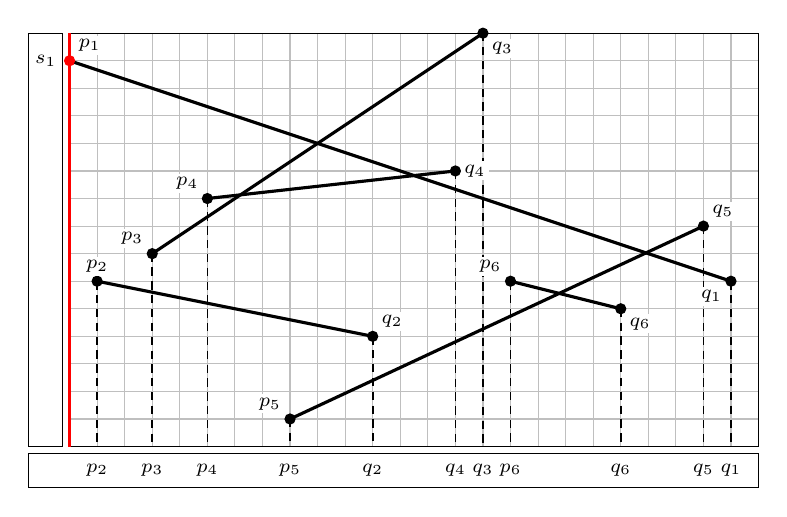
\begin{tikzpicture}[baseline=0]
            \tiktop
            
            -- line segments
            \foreach \start/\end in {
                P1S/P1E,
                P2S/P2E,
                P3S/P3E,
                P4S/P4E,
                P5S/P5E,
                P6S/P6E}
            {
                \draw[black,fill=black,line width=0.4mm]
                    (\start) -- (\end);
            }

            -- dashed lines
            \foreach \point in {
                    P1E,
                P2S,P2E,
                P3S,P3E,
                P4S,P4E,
                P5S,P5E,
                P6S,P6E}
            {
                \draw[black,line width=0.2mm, densely dashed]
                    let
                        \p1 = (\point)
                    in
                        (\x1, \y1) -- (\x1, 0);
            }

            -- sweep line
            \foreach \event in {P1S}
            {
                \draw[red,line width=0.4mm]
                    let
                        \p1 = (\event)
                    in 
                        (\x1, 0) -- (\x1, \ylines * \raster);
            }

            -- start- / end-point
            \foreach \point/\co in {
                P1S/red,P1E/black,
                P2S/black,P2E/black,
                P3S/black,P3E/black,
                P4S/black,P4E/black,
                P5S/black,P5E/black,
                P6S/black,P6E/black}
            {
                \draw[\co,fill=\co,line width=0.4mm]
                    (\point) circle (0.5mm);
            }

            -- events
            \foreach \event/\name/\i in {
                P1E/q/1,
                P2S/p/2,P2E/q/2,
                P3S/p/3,P3E/q/3,
                P4S/p/4,P4E/q/4,
                P5S/p/5,P5E/q/5,
                P6S/p/6,P6E/q/6}
            {
                \path
                    let
                        \p1 = (\event)
                    in 
                        node at (\x1,0) [below, fill=white, inner sep=1.25, outer sep=5] {$\scriptstyle \name_{\i} $};
            }

            -- status
            \foreach \start/\end/\i/\astart/\aend/\co in {
                P1S/P1E/1/above right/below left/red}
            {
                \path
                    let
                        \p1 = (\start),
                        \p2 = (\end)
                    in 
                        node at (0,\y1) [left, fill=white, inner sep=1.25, outer sep=3.5] {$\scriptstyle s_{\i} $};
            }

            -- start- / end-point text
            \foreach \point/\name/\i/\align/\co in {
                P1S/p/1/above right/black, P1E/q/1/below left/black,
                P2S/p/2/above/black,       P2E/q/2/above right/black,
                P3S/p/3/above left/black,  P3E/q/3/below right/black,
                P4S/p/4/above left/black,  P4E/q/4/right/black,
                P5S/p/5/above left/black,  P5E/q/5/above right/black,
                P6S/p/6/above left/black,  P6E/q/6/below right/black}
            {
                \node[\align, \co, fill=white, inner sep=1.25, outer sep=2] at (\point) {$\scriptstyle \name_{\i} $};
            }
            
        \end{tikzpicture}} &
        \setlength{\tabcolsep}{2pt}
        \makecell[l]{
        \begin{tabular}[t]{@{}llll@{}}
            Remove event    & $p_1$ & from  & $Q$ \\
            Add segment     & $s_1$ & to    & $S$ \\
            \multicolumn{4}{@{}l}{No upper or lower neighbours}
        \end{tabular} \\
        $
        \begin{aligned}[t]
            Q       &= \kq{ p_2, p_3, p_4, p_5, q_2, q_4, q_3, p_6, q_6, q_5, q_1 } \\
            S       &= \kq{ s_1 }
        \end{aligned}
        $} \\
        % --- LINE 3 --------------------------------------------------------
        \noindent\parbox[c][\pich]{\picb}{
        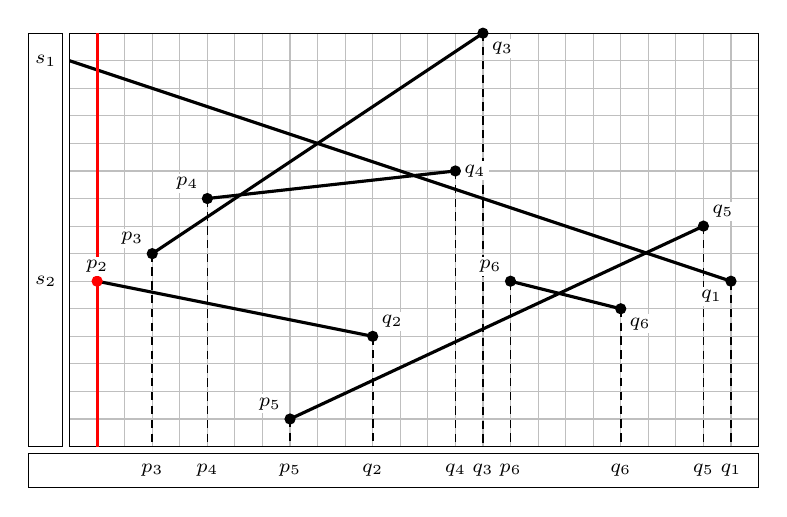
\begin{tikzpicture}[baseline=0]
            \tiktop

            -- line segments
            \foreach \start/\end in {
                P1S/P1E,
                P2S/P2E,
                P3S/P3E,
                P4S/P4E,
                P5S/P5E,
                P6S/P6E}
            {
                \draw[black,fill=black,line width=0.4mm]
                    (\start) -- (\end);
            }

            -- dashed lines
            \foreach \point in {
                    P1E,
                P2S,P2E,
                P3S,P3E,
                P4S,P4E,
                P5S,P5E,
                P6S,P6E}
            {
                \draw[black,line width=0.2mm, densely dashed]
                    let
                        \p1 = (\point)
                    in
                        (\x1, \y1) -- (\x1, 0);
            }

            -- sweep line
            \foreach \event in {P2S}
            {
                \draw[red,line width=0.4mm]
                    let
                        \p1 = (\event)
                    in 
                        (\x1, 0) -- (\x1, \ylines * \raster);
            }

            -- start- / end-point
            \foreach \point/\co in {
                P1E/black,
                P2S/red,P2E/black,
                P3S/black,P3E/black,
                P4S/black,P4E/black,
                P5S/black,P5E/black,
                P6S/black,P6E/black}
            {
                \draw[\co,fill=\co,line width=0.4mm]
                    (\point) circle (0.5mm);
            }

            -- events
            \foreach \event/\name/\i in {
                P1E/q/1,
                P2E/q/2,
                P3S/p/3,P3E/q/3,
                P4S/p/4,P4E/q/4,
                P5S/p/5,P5E/q/5,
                P6S/p/6,P6E/q/6}
            {
                \path
                    let
                        \p1 = (\event)
                    in 
                        node at (\x1,0) [below, fill=white, inner sep=1.25, outer sep=5] {$\scriptstyle \name_{\i} $};
            }

            -- status
            \foreach \start/\end/\i/\astart/\aend/\co in {
                P1S/P1E/1/above right/below left/red,
                P2S/P2E/2/above right/below left/red}
            {
                \path
                    let
                        \p1 = (\start),
                        \p2 = (\end)
                    in 
                        node at (0,\y1) [left, fill=white, inner sep=1.25, outer sep=3.5] {$\scriptstyle s_{\i} $};
            }


            -- start- / end-point text
            \foreach \point/\name/\i/\align/\co in {
                P1E/q/1/below left/black,
                P2S/p/2/above/black,       P2E/q/2/above right/black,
                P3S/p/3/above left/black,  P3E/q/3/below right/black,
                P4S/p/4/above left/black,  P4E/q/4/right/black,
                P5S/p/5/above left/black,  P5E/q/5/above right/black,
                P6S/p/6/above left/black,  P6E/q/6/below right/black}
            {
                \node[\align, \co, fill=white, inner sep=1.25, outer sep=2] at (\point) {$\scriptstyle \name_{\i} $};
            }
            
        \end{tikzpicture}} &
        \setlength{\tabcolsep}{2pt}
        \makecell[l]{
        \begin{tabular}[t]{@{}llll@{}}
            Remove event    & $p_2$ & from  & $Q$ \\
            Add segment     & $s_2$ & to    & $S$ below $s_1$ \\
            \multicolumn{4}{@{}l}{Check intersection:}
        \end{tabular} \\
        $
        \begin{aligned}[t]
            \text{above}       &= \kq{ s_1 } \\
            \text{below}       &= \kq{ \; }
        \end{aligned}
        $ \\
        $ \text{intersection}\kl{s_1, s_2} = \text{false} $ \\
        $
        \begin{aligned}[t]
            Q       &= \kq{ p_3, p_4, p_5, q_2, q_4, q_3, p_6, q_6, q_5, q_1 } \\
            S       &= \kq{ s_1, s_2 }
        \end{aligned}
        $} \\
        % --- LINE 4 --------------------------------------------------------
        \noindent\parbox[c][\pich]{\picb}{
        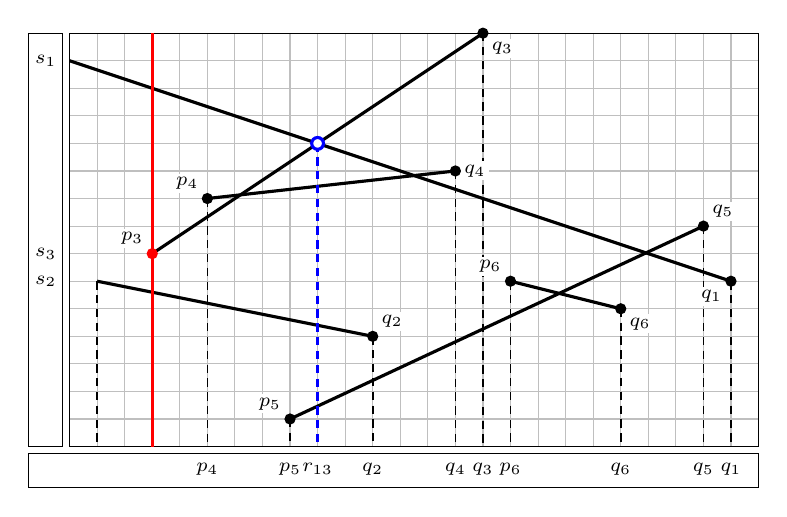
\begin{tikzpicture}[baseline=0]
            \tiktop
            -- line segments
            \foreach \start/\end/\i in {
                P1S/P1E/1,
                P2S/P2E/2,
                P3S/P3E/3,
                P4S/P4E/4,
                P5S/P5E/5,
                P6S/P6E/6}
            {
                \draw[black,fill=black,line width=0.4mm, name path global/.expanded=s\i]
                    (\start) -- (\end);
            }

            -- dashed lines
            \foreach \point in {
                    P1E,
                P2S,P2E,
                P3S,P3E,
                P4S,P4E,
                P5S,P5E,
                P6S,P6E}
            {
                \draw[black,line width=0.2mm, densely dashed]
                    let
                        \p1 = (\point)
                    in
                        (\x1, \y1) -- (\x1, 0);
            }

            -- sweep line
            \foreach \event in {P3S}
            {
                \draw[red,line width=0.4mm]
                    let
                        \p1 = (\event)
                    in 
                        (\x1, 0) -- (\x1, \ylines * \raster);
            }

            -- start- / end-point
            \foreach \point/\co in {
                P1E/black,
                P2E/black,
                P3S/red,P3E/black,
                P4S/black,P4E/black,
                P5S/black,P5E/black,
                P6S/black,P6E/black}
            {
                \draw[\co,fill=\co,line width=0.4mm]
                    (\point) circle (0.5mm);
            }

            -- intersection
            \path [name intersections={of=s1 and s3,by=r13}];
            \draw[blue,line width=0.4mm, densely dashed]
                    let
                        \p1 = (r13),
                    in
                        (\x1, \y1) -- (\x1, 0);
            \draw[blue, fill=white, line width=0.4mm]
                (r13) circle (0.75mm);

            -- events
            \foreach \event/\name/\i in {
                P1E/q/1,
                P2E/q/2,
                P3E/q/3,
                P4S/p/4,P4E/q/4,
                P5S/p/5,P5E/q/5,
                P6S/p/6,P6E/q/6,
                r13/r/13}
            {
                \path
                    let
                        \p1 = (\event)
                    in 
                        node at (\x1,0) [below, fill=white, inner sep=1, outer sep=5] {$\scriptstyle \name_{\i} $};
            }

            -- status
            \foreach \start/\end/\i/\astart/\aend/\co in {
                P1S/P1E/1/above right/below left/red,
                P2S/P2E/2/above right/below left/red,
                P3S/P3E/3/above left/below right/black}
            {
                \path
                    let
                        \p1 = (\start),
                        \p2 = (\end)
                    in 
                        node at (0,\y1) [left, fill=white, inner sep=1.25, outer sep=3.5] {$\scriptstyle s_{\i} $};
            }

            -- start- / end-point text
            \foreach \point/\name/\i/\align/\co in {
                P1E/q/1/below left/black,
                P2E/q/2/above right/black,
                P3S/p/3/above left/black,  P3E/q/3/below right/black,
                P4S/p/4/above left/black,  P4E/q/4/right/black,
                P5S/p/5/above left/black,  P5E/q/5/above right/black,
                P6S/p/6/above left/black,  P6E/q/6/below right/black}
            {
                \node[\align, \co, fill=white, inner sep=1.25, outer sep=2] at (\point) {$\scriptstyle \name_{\i} $};
            }
            
        \end{tikzpicture}} &
        \setlength{\tabcolsep}{2pt}
        \makecell[l]{
        \begin{tabular}[t]{@{}llll@{}}
            Remove event    & $p_3$ & from  & $Q$ \\
            Add segment     & $s_3$ & to    & $S$ between $s_1$ and $s_2$ \\
            \multicolumn{4}{@{}l}{Check intersection:} \\
            above           & \multicolumn{3}{@{}l}{$= \kq{ s_1 }$} \\
            below           & \multicolumn{3}{@{}l}{$= \kq{ s_2\; }$} \\
            intersection$\kl{s_1, s_3}$   & \multicolumn{3}{@{}l}{$=$ true $\to	\textcolor{blue}{r_{13}}$} \\
            intersection$\kl{s_2, s_3}$   & \multicolumn{3}{@{}l}{$=$ false }
        \end{tabular} \\
        $
        \begin{aligned}[t]
            Q       &= \kq{ p_4, p_5, q_2, q_4, q_3, p_6, q_6, q_5, q_1 } \\
            S       &= \kq{ s_1, s_3, s_2 }
        \end{aligned}
        $} \\
        
   \end{tabularx}
\end{document}